\documentclass{beamer}

\usepackage{adjustbox}
\usepackage{listings}
\usepackage{graphicx}
\usepackage{mathtools}
\usepackage{tikz}

\usetikzlibrary{calc,trees,positioning,arrows,chains,shapes.geometric,%
                decorations.pathreplacing,decorations.pathmorphing,shapes,%
                matrix,shapes.symbols}

\tikzset{
    >=stealth',
    punktchain/.style={
        rectangle,
        rounded corners,
        draw=black, very thick,
        text width=10em,
        minimum height=3em,
        text centered,
        on chain
    },
    line/.style={draw, thick, <-},
    element/.style={
        tape,
        top color=white,
        bottom color=blue!50!black!60!,
        minimum width=8em,
        draw=blue!40!black!90, very thick,
        text width=10em,
        minimum height=3.5em,
        text centered,
        on chain
    },
    every join/.style={->, thick, shorten >=1pt},
    decoration={brace},
    tuborg/.style={decorate},
    tubnode/.style={midway, right=2pt}
}

\begin{document}
    \title{Demystifying Haskell}
    \subtitle{An in-depth examination of the Fibonacci sequence.}
    \author{Andrew Rademacher}

    \definecolor{dkgreen}{rgb}{0,0.6,0}
    \definecolor{gray}{rgb}{0.5,0.5,0.5}
    \definecolor{mauve}{rgb}{0.58,0,0.82}

    \lstdefinelanguage{JavaScript}{
        keywords={typeof, new, true, false, catch, function, return, null, catch, switch, var, if, in, while, do, else, case, break},
        keywordstyle=\color{blue}\bfseries,
        ndkeywords={class, export, boolean, throw, implements, import, this},
        ndkeywordstyle=\color{darkgray}\bfseries,
        identifierstyle=\color{black},
        sensitive=false,
        comment=[l]{//},
        morecomment=[s]{/*}{*/},
        commentstyle=\color{purple}\ttfamily,
        stringstyle=\color{red}\ttfamily,
        morestring=[b]',
        morestring=[b]"
    }

    \lstset{frame=tb,
        language=JavaScript,
        aboveskip=3mm,
        belowskip=3mm,
        showstringspaces=false,
        columns=flexible,
        basicstyle={\small\ttfamily},
        numbers=none,
        numberstyle=\tiny\color{gray},
        keywordstyle=\color{blue},
        commentstyle=\color{dkgreen},
        stringstyle=\color{mauve},
        breaklines=true,
        breakatwhitespace=true
        tabsize=3
    }

% FRAME:TITLE
    \frame{\titlepage}

% FRAME:FIBONACCI
    \begin{frame}
        \frametitle{The Fibonacci Sequence}

        \begin{columns}[c]
            \begin{column}[T]{5cm}
                \begin{itemize}
                    \item Sequence is infinite
                    \item Sequence is self-referencing
                    \item Values grow exponentially
                    \item Values are always positive
                \end{itemize}
            \end{column}
            \begin{column}[T]{5cm}
                \begin{figure}
                    \centering
                    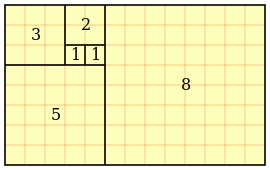
\includegraphics[height=3cm]{./fibs/images/FibonacciBlocks.png}
                \end{figure}

                \begin{figure}
                    \centering
                    \begin{math}
                        \left\{1,1,2,3,5,8...\right\}
                    \end{math}
                \end{figure}
               
                \begin{figure}
                    \centering
                    \begin{math}
                        F_{n} = F_{n-1} + F_{n-2}
                    \end{math}
                \end{figure}
            \end{column}
        \end{columns}
    \end{frame}

% FRAME:JAVASCRIPT
    \lstset{language=JavaScript}
    \begin{frame}[fragile=singleslide]
        \frametitle{Traditional JavaScript Implementation}

        \begin{lstlisting}
        function getFibs (n) {
            var fibs = [1, 1];
            for (var i = 2; i < n; i++) 
                fibs.push(fibs[fibs.length - 1] + fibs[fibs.length - 2]);

            return fibs;
        }
        \end{lstlisting}
    \end{frame}

% FRAME:JAVA
    \lstset{language=Java}
    \begin{frame}[fragile=singleslide]
        \frametitle{Traditional Java Implementation}
        
        \begin{lstlisting}
        public static BigInteger[] getFibs(int n) {
            BigInteger[] fibs = new BigInteger[n];
            fibs[0] = BigInteger.valueOf(1);
            fibs[1] = BigInteger.valueOf(1);
            for (int i = 2; i < n; i++)
                fibs[i] = fibs[i - 1].add(fibs[i - 2]);

            return fibs;
        }
        \end{lstlisting}
    \end{frame}

% FRAME:PROCESS
    \begin{frame}[fragile=singleslide]
        \frametitle{Imperative Process}
        
        \adjustbox{scale=0.5}{
            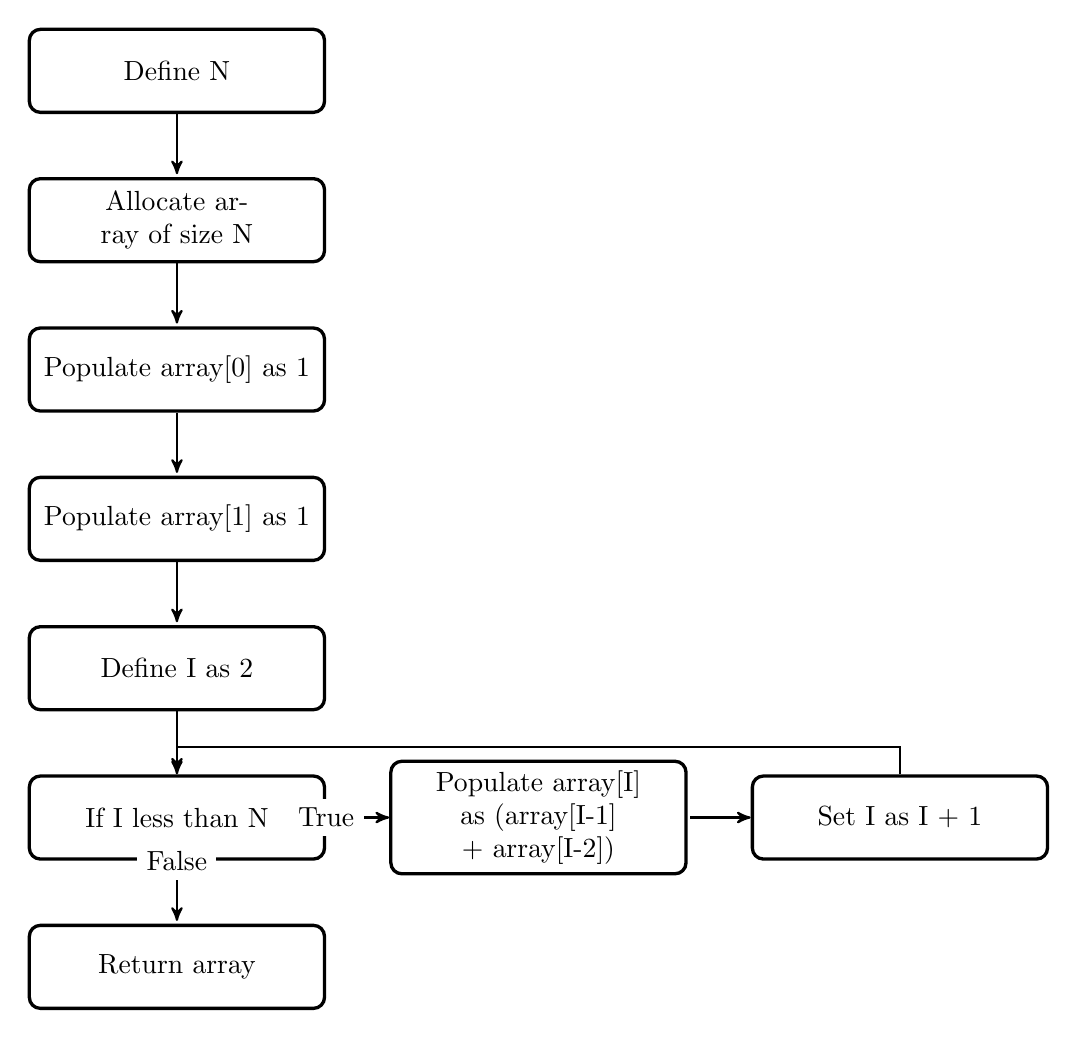
\begin{tikzpicture}[node distance=0.8cm,start chain=going below]
                \node[punktchain, join] (defineN) {Define N};
                \node[punktchain, join] (alloc) {Allocate array of size N};
                \node[punktchain, join] (pop0) {Populate array[0] as 1};
                \node[punktchain, join] (pop1) {Populate array[1] as 1};
                \node[punktchain, join] (defineI) {Define I as 2};
                
                \node[punktchain, join] (if) {If I less than N};
                \begin{scope}[start branch=venstre, every join/.style={->, thick, shorten <=1pt}]
                    \node[punktchain, on chain=going right, join=by {->}] 
                        (popI) {Populate array[I] as (array[I-1] + array[I-2])};
                    \node[punktchain, on chain=going right, join=by {->}]
                        (setI) {Set I as I + 1};
                \end{scope}
                
                \node[punktchain, join] (return) {Return array};

                % -- Post processing -- %

                \draw (if.east) node [fill=white] {True};
                \draw[|-,-|,->,thick] (setI.north) |-+(0,1em)-| (if.north);
                \draw (if.south) node [fill=white] {False};
            \end{tikzpicture}
        }
    \end{frame}

% FRAME:HASKELL
    \lstset{language=Haskell}
    \begin{frame}[fragile=singleslide]
        \frametitle{New Fangled Haskell Implementation}

        \begin{lstlisting}
        fibs = 1 : 1 : [ a + b | (a, b) <- zip fibs (tail fibs) ]
        \end{lstlisting}
    \end{frame}

% FRAME:WHAT
    \begin{frame}[fragile=singleslide]
        \frametitle{What just happened?}

        \begin{figure}
            \centering
            
\includegraphics[scale=0.35]{./fibs/images/lolwutpear.jpg}
        \end{figure}
    \end{frame}

% FRAME:ASSIGNMENT
    \lstset{language=Haskell}
    \begin{frame}[fragile=singleslide]
        \frametitle{Values != Variables}

        \begin{columns}[c]
            \begin{column}[T]{5cm}
                \begin{itemize}
                    \item Haskell has no variables
                    \item Values can be bound to a name
                    \item Values can only be assigned once
                    \item Values never change
                \end{itemize}
            \end{column}
            \begin{column}[T]{5cm}
                \begin{lstlisting}
                fibs = 1 // Valid assignment
                fibs = 2 // Invalid assignment
                \end{lstlisting}
            \end{column}
        \end{columns}
    \end{frame}

% FRAME:LISTS
    \begin{frame}[fragile=singleslide]
        \frametitle{Lists}

        \begin{columns}[c]
            \begin{column}[T]{5cm}
            \end{column}
            \begin{column}[T]{5cm}
            \end{column}
        \end{columns}
    \end{frame}
\end{document}
